%%%%%%%%%%%%%%%%%%%%%%%%%%%%%%%%%%%%%%%%%%%%%%%%%%%%%
%			HLAVIČKA								%
%%%%%%%%%%%%%%%%%%%%%%%%%%%%%%%%%%%%%%%%%%%%%%%%%%%%%
\documentclass[openany,12pt]{memoir}

\usepackage[utf8]{inputenc} 
\usepackage[czech]{babel}
\usepackage[T1]{fontenc}
\usepackage[top=1cm, bottom=2cm, left=2cm, right=2cm]{geometry}  % --> NASTAVENÍ OKRAJŮ
\usepackage{fancyhdr}
\usepackage{graphicx}
\usepackage{lmodern}
\usepackage{xwatermark}
\usepackage{xcolor}
\usepackage{changepage}




%%%%%% Package na zpěvník
\usepackage[full]{leadsheets}%http://mirrors.nic.cz/tex-archive/macros/latex/contrib/leadsheets/leadsheets_en.pdf   --> dokumentace	
\definesongtitletemplate{empty}{} 
\setchords{
format = \bfseries,   %tučné akordy
minor = {mi},% 
input-notation = {german},%
output-notation = {german}%
}
\definesongtitletemplate{empty}{} 

\newlength{\drop}
\newwatermark[allpages,color=red!50,angle=0,scale=2, xpos=0,ypos=0]{
\includegraphics[width=5cm]{obr/pozadi.jpg}} %--> dvojka na pozadí


%%%% Vlastní příkazy
\newcounter{Slokočet}   %Automatické číslování slok
\newcommand{\mezera}{\vspace*{0.5cm}}   %Horizontální odsazení slok
\newcommand{\stred}{5.2cm}   %%% Na zarovnání slok doprostřed, pozn. automatičtější zarovnávání na střed nejde
\newcommand{\refren}{\mezera \noindent \textbf{R:} } %refrén
\newcommand{\sloka}{\mezera \noindent \addtocounter{Slokočet}{1} \arabic{Slokočet}. } 	%sloka, která se automaticky čísluje
\newcommand{\ssloka}{\mezera \noindent}  % vlastní číslo sloky


%%%%%%%%%%%%%%%%%%%%%%%%%%%%%%%%%%%%%%%%%%%%%%%%%%%%%%
%			NÁVOD									 %
%%%%%%%%%%%%%%%%%%%%%%%%%%%%%%%%%%%%%%%%%%%%%%%%%%%%%%
%1. Věci v hlavičce IGNOROVAT
%2. Píseň psát do prostoru mezi \begin{song} a \end{song}
%3. další řádek se značí dvěma odsazeníma (= dvakrát stisknout enter)
%4. \refren vždy na začátku refrenu a \sloka na začátek sloky (automaticky se čísluje)
%  \ = alt gr + q ; [/] = alt gr f/g ; {/} = alt gr + b/n; ^ = alt gr + 3 + mezera
%Cokoliv napíšete do ^{  } se bude brát jako akord
%když se toto bude dotýkat nějakého slova (nebude mezi tím a slovem mezera)
%tak se akordy zjeví nad slovem, ale pište to před slovo
%Když se to nedotýká slova, tak akord lítá ve vzduchu a vytiskne se větší mezera
%První možnost je asi preferovanější
%5. Akordy stačí psát jen do první sloky, když se nezmění -- kytaristi to zvládnou



%<++>
%\usepackage{subfiles}
%</++>

\begin{document}

\pagestyle{empty}
%\addtocontents{toc}{\protect\thispagestyle{empty}}
\tableofcontents \thispagestyle{empty}\newpage
\newgeometry{top=1.5cm, bottom = 0cm, left = 2cm, right = 2cm}

\pagestyle{simple}
\addcontentsline{toc}{section}{Skaustká hymna a Večerka}%\documentclass[../main.tex]{subfiles}

\begin{song}{title=\centering Skautská hymna \\\normalsize  \vspace*{-0.3cm}}  %% sem se napíše jméno songu a autor
\moveright 6cm \vbox{      %Varianta č. 1  ---> Jeden sloupec zarovnaný na střed	
\textcolor{white}{something}


^{D}Junáci ^{G}vzhůru, ^{D}volá den,

luh ^{Hmi}květem ^{G}kývá, ^{A}orosen,

sluníčko blankytem pílí,

před ^{Emi}námi pouť ^{F#m}vede k ^{A}cíli.

^{D}Junáci ^{G}vzhůru ^{D}volá den,

^{G}junáci ^{D G}vzhůru ^{A}volá ^{D}den. 

}
\setcounter{Slokočet}{0}
\end{song}

\vspace*{7cm}
\begin{song}{title=\centering Večerka \vspace*{-0.3cm}}
\moveright 6.2cm \vbox{      %Varianta č. 1  ---> Jeden sloupec zarovnaný na střed	

\sloka
 Zapad den, slunce svit,
 
 vymizel z údolí,
 
 z temen hor odpočiň
 
 každý kdos boží tvor.
 
\sloka
 V lese klín padl stín,
 
 hasne již vatry zář,
 
 svatý mír kráčí z hor,
 
 usíná boží tvor.
 
\sloka
BRUMENDO
}
\setcounter{Slokočet}{0}
\end{song}

\newpage
\addcontentsline{toc}{section}{1. signální}\begin{song}{title=\centering 1. signální \\\normalsize Chinaski  \vspace*{-0.3cm}}  %% sem se napíše jméno songu a autor
\moveright \stred \vbox{      %Varianta č. 1  ---> Jeden sloupec zarovnaný na střed	

\sloka 
	^{Emi}Až si ^{G}zejtra ráno ^{C}řeknu zase 

	^{Emi}jednou provždy dost,

	^{G}právem se mi ^{C}budeš tiše ^{Emi}smát

	jak omluvit si svoji slabost,

	nenávist a zlost,

	když za všechno si můžu vlastně sám. 

\refren
	^{Ami}Za spoustu dní možná za ^{C}spoustu let 

	až se mi ^{G}rozední, budu ti ^{D}vyprávět 

	na 1.signální, jak jsem vobletěl svět, 

	jak tě to vomámí a nepustí zpět.

	Jaký si to ^{F}uděláš, ^{B}takový to ^{Dmi}máš. 

	Jaký si to ^{F}uděláš, ^{B}takový to ^{Dmi}máš. 

\sloka
	Až se dneska večer budu tvářit
	
	zas jak Karel Gott, 
	
	budu zpívat vampamtydapam,
	
	všechna sláva polní tráva,
	
	ale peníz přijde vhod,
	
	jak jsem si to uďál tak to mám.

\refren

\sloka Nana\dots

}
\setcounter{Slokočet}{0}
\end{song}


\newpage
\addcontentsline{toc}{section}{Cestou do Jenkovic}\begin{song}{title=\centering Cestou do Jenkovic \\\normalsize Radůza  \vspace*{-0.3cm}}  %% sem se napíše jméno songu a autor
\moveright 3cm \vbox{      %Varianta č. 1  ---> Jeden sloupec zarovnaný na střed	

\sloka 
	^{D}Můj děda z kola ^{Hmi{\color{white}aaa}}seskočil, ^{C{\color{white}aa}}před prázdnou kašnou ^{A}na náměstí. 
	
	^{D}Na lavičce chleba ^{Hmi{\color{white}aaa}}posvačil, ^{C{\color{white}aaaa}}seřídil hodinky ^{A}na zápěstí.

\refren ^{D}A čápi z komína ^{A}od cihelny, zobákem ^{C{\color{white}aaaaa}}klapou, asi jsou ^{G{\color{white}aaaaaa}}nesmrtelný.

\sloka 
	Tři kluci v bílejch košilích dělili se o poslední spartu,

	ze zídky do záhonu skočili, přeběhli ulici a zmizeli v parku.

\refren 

\sloka 
	V oknech svítěj peřiny, na bílý kafe mlíko se vaří, 

	teď právě začaly prázdniny, venku je teplo a všechno se daří.

\refren



}
\setcounter{Slokočet}{0}
\end{song}


\begin{figure}[h]
\centering
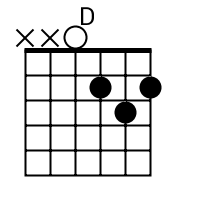
\includegraphics[width=3cm]{../Akordy/d.png}
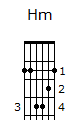
\includegraphics[width=3cm]{../Akordy/hm.png}
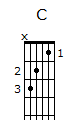
\includegraphics[width=3cm]{../Akordy/c.png}
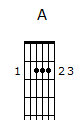
\includegraphics[width=3cm]{../Akordy/a.png}
\end{figure}
\newpage
\addcontentsline{toc}{section}{Cestou od hřbitova}\begin{song}{title=\centering Cestou od hřbitova \\\normalsize Znouzecnost  \vspace*{-0.3cm}}  %% sem se napíše jméno songu a autor
\moveright 4.2cm \vbox{      %Varianta č. 1  ---> Jeden sloupec zarovnaný na střed	

\sloka
	^{G{\color{white}aaa}}Cestou od hřbitova ^{D{\color{white}aaa}}potkal jsem tu madam,
	
	^{F}slzy se jí pod závojem ^{G{\color{white}aa}}derou do očí,
	
	ňáká mladá vdova -- ^{D}tak upřímnou soustrast
	
	^{F{\color{white}aaaa}}popřeju jí na začátek ^{G}a už se to točí.
	
\refren 
	Laj laj \dots \textbf{G, D, F, G, D, F, G}

	/: ^{G{\color{white}aa}}Svět, svět se ^{D{\color{white}aaaa}}zatočí a ^{F{\color{white}aa}}život jde ^{G}dál. :/ %Zatočí nebo točí? Já bych řekl, že zatočí, Ano, ztoci

\sloka
	Proč ty slzy, madam, vždyť žijem tak krátce,
	
	žal ve vaší tváři k vašemu já neladí.
	
	Nabízím Vám rámě -- služebník a rádce
	
	a kašlete na ty řeči, že se to nehodí.

\refren

\sloka
	Budu Vám číst z dlaní, co vás ještě čeká,
	
	něžně a s pietou vaše slzy osuším.
	
	Cestou od hřbitova jen chviličku váhá
	
	a ten pod tou hlínou už stejně nic netuší.

\refren

\sloka
	Balím holky na hřbitově přes duchovní útěchu,
	
	no a potom cestou domů skončí u mě v pelechu.
	
	Jsem dle řečí na pavlači amorální dobytek.
	
	A můj názor na celou věc: Oboustrannej užitek!

\refren


}
\setcounter{Slokočet}{0}
\end{song}


\newpage
\addcontentsline{toc}{section}{Černej pasažér}\input{../songy/Cernejpasazer}\newpage
\addcontentsline{toc}{section}{Černobílý svět}%../main.tex]{subfiles}

\begin{song}{title=\centering Černobílý svět \\\normalsize Totální nasazení \vspace*{-0.3cm}}
%\vspace*{-1.2cm}
\moveright \stred \vbox{      %Varianta č. 1  ---> Jeden sloupec zarovnaný na střed
\setcounter{Slokočet}{0}
\sloka
^{Dmi}Jsme loutky ^{F}bez nití

^{B}já i všech ^{C{\color{white}\_\_\_}}patnáct druhů ^{Dmi}mých.

Bez smrti ^{F}bez žití

^{B{\color{white}\_\_\_\_}}bloumáme ^{C{\color{white}\_}}tupě po polích.

\refren
^{Dmi}Černá a ^{B{\color{white}\_}}bílá je,

^{C{\color{white}\_}}osm kroků tam a osm^{Dmi}sem,

frontová ^{B{\color{white}\_}}linie.

^{C}Na věky proti sobě ^{Dmi}jdem.

\sloka
^{Dmi}Stojí tu ^{F{\color{white}\_\_}}opodál

^{B}náš ^{{\color{white}\_\_\_}C}domnělý to ^{{\color{white}\_\_}Dmi}nepřítel.

I když jsem ^{F{\color{white}\_}}černý král

^{B{\color{white}\_\_}}nejsem svých ^{C\,\,\,\,}figur ^{{\color{white}\_}Dmi}velitel.

\sloka
Vždy první na tahu

jsem ten kdo bitvu rozpoutá,

ač nemá odvahu.

Bílý a nešťastný jsem král

\refren

\sloka
Přestal jsem počítat,

kolikrát jsem padnul a zas vstal,

kolikrát dostal mat,

útočil nebo utíkal

\sloka
Jsme jenom figury

ať král či pěšák beze jména

a hraní na vojáky je vaše lidská doména.

\refren

}
\end{song}
\setcounter{Slokočet}{0}
\newpage
\addcontentsline{toc}{section}{Dej mi víc své lásky}\begin{song}{title=\centering Dej mi víc své lásky \\\normalsize Olympic  \vspace*{-0.3cm}}  %% sem se napíše jméno songu a autor
\moveright \stred \vbox{      %Varianta č. 1  ---> Jeden sloupec zarovnaný na střed	

\sloka
	^{Emi{\color{white}\_\_}}Vymyslel jsem spoustu napadů, ^{G}aů,
   
	co ^{Emi{\color{white}\_\_}}podporujou hloupou ^{{\color{white}\_}D}náladu, ^{H7}aů,

	^{Emi}hodit klíče do kanálu, ^{A}sjet po zadku ^{Ami}holou skálu,

	v ^{Emi}noci chodit ^{H7\,\,\,\,}strašit do ^{{\color{white}\_}Emi}hradu, aů.

\sloka
	Dám si dvoje housle pod bradu, aů,

	v bílé plachtě chodím pozadu, aů,
	
	úplně melancholicky, s citem pro věc jako vždycky

	vyrábím tu hradní záhadu, aů.

\refren
	^{G}Má drahá, dej mi víc, ^{H7}má drahá, dej mi víc,

	^{Emi}má drahá, ^{C}dej mi víc své ^{G{\color{white}\_\_}}lásky, ^{D7}aů,

	^{G}já nechci skoro nic, ^{H7}já nechci skoro nic,

	^{Emi}já chci jen ^{C{\color{white}\_\_\_}}pohladit tvé ^{G{\color{white}\_\_}}vlásky, ^{H7}aů.

\sloka
	Nejlepší z těch divnejch nápadů, aů,
	
	mi dokonale zvednul náladu, aů,

	natrhám ti sedmikrásky, tebe celou s tvými vlásky

	zamknu si na sedm západů, aů.

\refren

\sloka = 3.


}
\setcounter{Slokočet}{0}
\end{song}



\newpage
\addcontentsline{toc}{section}{Do Ameriky}\documentclass[../main.tex]{subfiles}

\chapter*{Do Ameriky}

\noindent\hspace{0.15\linewidth}
\begin{minipage}{0.7\linewidth}
\begin{song}{title=Do Ameriky}

\begin{verse}[numbered]
	^{D}Do Ameriky jezděj Parníky,\\
	když tam přijdeš, zdá se ti to ^{A7}všecko veliký,\\
	^{\phantom{S}}je to fakticky tuze praktický  \\
	když tam přijdeš, umět anglic^{D}ky. \\
\end{verse}

\begin{verse*}
	Refrain:
	^{D}Dobrou noc - good night, ^{A7}výborně - all right,\\
	Konrád White, už je off^{D}side (housemister - Dally sister!) \\
	^{D}Dneska je today, ^{A7}dobrý den - good day,\\
	já jsem byl taky chu^{D}dej. \\ 
	^{G}His Master's Voice, Yankee Doo^{G}dle,\\ \\
	^{En7}máš apetit? (mám) ^{A7}vem si štrůdl! (do pusy)\\
	^{D}Sto kilo je cent, ^{A7}patent je patent,\\
	husa v troubě happy^{D}end.
\end{verse*}

\begin{verse}[numbered]
	Co Buffalo Bill vrazil do kobyl,\\
	za to by si bejval byl koupil automobil,\\
	cowboy na koni už se nehoní,\\
	přestože mu Fordka nevoní.\\
\end{verse}

\begin{verse*}
	Refrain
\end{verse*}

\begin{verse}[numbered]
	Mám na západě chajdu v Nevadě,\\
	zlatou žílu v Arizoně, doly v Kanadě,\\
	babička na mě šetří v Panamě\\
	a já si tu žiju náramě!\\
\end{verse}



\end{song}

\end{minipage}\newpage
\addcontentsline{toc}{section}{Do dne a do roka}\input{../songy/Dodneadoroka}\newpage
\addcontentsline{toc}{section}{Dokud se zpívá}\begin{song}{title=\centering Dokud se zpívá \\\normalsize Jaromír Nohavica  \vspace*{-0.3cm}}  %% sem se napíše jméno songu a autor
\moveright 3.8cm \vbox{      %Varianta č. 1  ---> Jeden sloupec zarovnaný na střed	

\sloka 
	^{C}Z Těšína ^{Emi\,\,\,\,\,}vyjíždí ^{Dmi7}vlaky co ^{F{\color{white}aaaaaa}C}čtvrthodinu, ^{Emi\,Dmi7\,G}

	včera jsem nespal a ani dnes nespočinu,

	^{F}svatý ^{G}Medard, můj ^{C}patron, ťuká ^{Ami}si na ^{{\color{white}aa}G}čelo,

	ale ^{F}dokud se ^{G}zpívá, ^{F}ještě se ^{G{\color{white}aaaa}C}neumřelo. ^{Emi\,Dmi7\,G}

\sloka
	Ve stánku koupím si housku a slané tyčky,
	
	srdce mám pro lásku a hlavu pro písničky,
	
	ze školy dobře vím, co by se dělat mělo,
	
	ale dokud se zpívá, ještě se neumřelo.

\sloka
	Do alba jízdenek lepím si další jednu,
   
	vyjel jsem před chvílí, konec je v nedohlednu,
	
	za oknem míhá se život jak leporelo,
	
	ale dokud se zpívá, ještě se neumřelo.

\sloka
	Stokrát jsem prohloupil a stokrát platil draze,
	
	houpe to, houpe to na housenkové dráze,
	
	i kdyby supi se slítali na mé tělo,
	
	tak dokud se zpívá, ještě se neumřelo.

\sloka
	Z Těšína vyjíždí vlaky až na kraj světa,
	
	zvedl jsem telefon a ptám se: \uv{Lidi, jste tam?}
	
	A z veliké dálky do uší mi zaznělo,
	
	/: že dokud se zpívá, ještě se neumřelo. :/


}
\setcounter{Slokočet}{0}
\end{song}
\newpage
\addcontentsline{toc}{section}{Franky Dlouhán}\begin{song}{title=\centering Franky Dlouhán \\\normalsize Brontosauři  \vspace*{-0.3cm}}  %% sem se napíše jméno songu a autor
\moveright \stred \vbox{      %Varianta č. 1  ---> Jeden sloupec zarovnaný na střed	

\sloka 
	^{C}Kolik je smutného,
	
	když ^{F} mraky černé ^{C}jdou

	lidem nad ^{G}hlavou ^{F}smutnou dálavo^{C}u.
	
	Já slyšel příběh, který velkou pravdu měl,
	
	za čas odletěl, každý zapomněl.

\refren
	^{C}Měl kapsu ^{G}prázdnou Franky Dlouhán,

	po státech ^{F}toulal se jen ^{C}sám, a že

	byl ^{F}veselej, tak ^{C}každej měl ho ^{G7}rád.

	Tam ruce k ^{F}dílu mlčky přiloží a ^{C}zase

	jede ^{Ami}dál. A ^{F}každej kdo s ním

	^{G}chvilku byl, tak ^{F}dlouho ^{G7}se pak ^{C}smál.
	
\sloka	
	Tam, kde byl pláč, tam Franky hezkou píseň měl,
	
	slzy neměl rád, chtěl se jenom smát.
	
	A když pak večer ranče tiše usínaj,
	
	Frankův zpěv jde dál nocí s písní dál.\elipsa\dots
	
\sloka
	Tak Frankyho vám jednou našli, přestal žít,
	
	jeho srdce spí, tiše smutně spí.
	
	Bůh ví jak, za co tenhle smíšek konec měl,
	
	farář píseň pěl, umíraček zněl.\elipsa\dots

}
\setcounter{Slokočet}{0}
\end{song}


\begin{figure}[h]
\centering
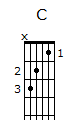
\includegraphics[width=3cm]{../Akordy/c.png}
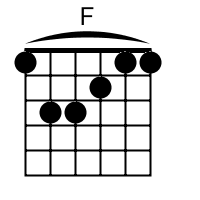
\includegraphics[width=3cm]{../Akordy/f.png}
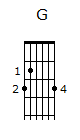
\includegraphics[width=3cm]{../Akordy/g.png}
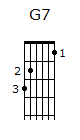
\includegraphics[width=3cm]{../Akordy/g7.png}
\end{figure}
	\newpage 
\addcontentsline{toc}{section}{God's Gonna Cut You Down}\documentclass[../main.tex]{subfiles}

\chapter{God's gonna cut you down}

\noindent\hspace{0.15\linewidth}\begin{minipage}{0.7\linewidth}
\begin{song}{title=Johnny Cash - Gods gonna cut you down}
\begin{verse}[numbered]
You^{Am} can run on for a long time, \\
Run^{Am} on for a long time, \\
Run^{Am} on for a long time, \\
Sooner, or later^{Dm}, God'll cut you down^{Am}. \\
Sooner, or later^{Dm}, God'll cut you down^{Am}. \\
\end{verse}
\begin{verse}[numbered]
Go and tell^{Am} that long tongue liar, \\
Go and tell^{Am} that midnight rider, \\
Tell the rambler^{Am}, the gambler, the back biter, \\
Tell^{C} 'em that God's^{Em} gonna cut^{Am} 'em down. \\
Tell^{C} 'em that God's^{Em} gonna cut^{Am} 'em down. \\
\end{verse}
\begin{verse}[numbered]
Well my^{Am} goodness gracious, let me tell you the news. \\
My heads^{Am} been wet with the midnight dew. \\
I've^{Am} been down on bended knee, \\
talkin^{Am} to the man from Galiee. \\
He spoke^{Am} to me in a voice so sweet, \\
I thought^{Am} I heard the shuffle of angels feet.  \\
He called^{Am} my name and my heart stood still,  \\
When He^{Am} said^{Mute} \uv{John go do my will}  \\
\end{verse}
\begin{verse}[numbered]
Go and tell^{Am} that long tongue liar, \\
Go and tell^{Am} that midnight rider, \\
Tell the rambiler^{Am}, the gambler, the back biter, \\
Tell^{C} 'em that God's^{Em} gonna cut 'em down^{Am}. \\
Tell^{C} 'em that God's^{Em} gonna cut 'em down^{Am}. \\
\end{verse}
\end{song}
\end{minipage}

\newpage
\vspace*{4.5cm}
\noindent\hspace{0.15\linewidth}\begin{minipage}{0.7\linewidth}
\begin{song}{title=Johnny Cash - Gods gonna cut you down}
\begin{verse}
\item[5.]You can run^{Am} on for a long time, \\
Run^{Am} on for a long time, \\
Run^{Am} on for a long time, \\
Sooner^{C}, or later,^{Em} God'll cut^{Am} you down. \\
Sooner^{C}, or later,^{Em} God'll cut^{Am} you down. \\
You may throw^{Am} your rock, hide your hand, \\
Workin^{Am} in the dark against your fellow man. \\
But as^{Am} sure as God made black and white, \\
What's done^{Am} in the dark, will be brought to the light. \\
\end{verse}
\begin{verse}
\item[6.]You can run^{Am} on for a long time, \\
Run^{Am} on for a long time, \\
Run^{Am} on for a long time, \\
Sooner^{C}, or later,^{Em} God'll cut^{Am} you down. \\
Sooner^{C}, or later,^{Em} God'll cut^{Am} you down. \\
\end{verse}
\begin{verse}
\item[7.]Go and tell^{Am} that long tongue liar, \\
Go and tell^{Am} that midnight rider, \\
Tell the rambler^{Am}, the gambler, the back biter, \\
Tell^{C} 'em that God's^{Em} gonna cut^{Am} 'em down. \\
Tell^{C} 'em that God's^{Em} gonna cut^{Am} 'em down^{Am}. \\
Tell^{C} 'em that God's^{Em} gonna cut^{Am} 'em down^{Am}. 
\end{verse}
\end{song}
\end{minipage}

\newpage %!!! Akordy dát nad nad slova, vyřadit opakující se akordy
\addcontentsline{toc}{section}{Hallelujah}\begin{song}{title=\centering Hallelujah \\\normalsize Leonard Cohen / Jeff Buckley \vspace*{-0.3cm}}  %% sem se napíše jméno songu a autor

\fontsize{11pt}{12pt}\selectfont

\moveright 1cm \vbox{      %Varianta č. 1  ---> Jeden sloupec zarovnaný na střed
\begin{minipage}[t]{0.48\textwidth}\setlength{\parindent}{0.25cm}  %Varianta č. 2 --> Dva sloupce

\sloka
	I ^{C}heard there was a ^{Am}secret chord  
	
	That ^{C}David played and it ^{Am}pleased the lord  
	
	But ^{F}you don't really ^{G}care for music, ^{C}do you?^{G}  
	
	Well ^{C}it goes like this the ^{F}fourth, the ^{G}fifth  
	
	The ^{Am}minor fall and the ^{F}major lift  
	
	The ^{G}baffled king ^{E7}composing halle^{Am}lujah  
	

\refren
^{F}Hallelujah, ^{Am}hallelujah, ^{F}hallelujah,

 ^{C}halleluuu - u - ^{G}uuu - u - ^{C}jah \dots 

\sloka
	Your faith was strong, but you needed proof,  
	
	you saw her bathing on the roof,  
	
	her beauty and the moonlight overthrew you.  
	
	She tied you to a kitchen chair,  
	
	she broke your throne, and she cut your hair,  
	
	and from your lips she drew the Hallelujah!  


\refren


\sloka
	You say I took the name in vain,  
	
	I don't even know the name,  
	
	but if I did, well really, what's it to you?  
	
	There's a blaze of light in every word,  

	it doesn't matter which you heard,  
	
	the holy or the broken Hallelujah!  
	

\refren

\sloka
	Baby, I've been here before,  
	
	I know this room, I've walked this floor,  
	
	I used to live alone before I knew you.  
	
	I've seen your flag on the marble arch,  
	
	but love is not a victory march,  
	
	it's a cold and it's a broken Hallelujah!  


\end{minipage}\begin{minipage}[t]{0.48\textwidth}\setlength{\parindent}{0.45cm}  % V případě varianty č.2 jde odsud text do pravé části
\vspace*{0.6cm}
\refren

\sloka
	There was a time you let me know,   
	
	what's really going on below,   
	
	but now you never show it to me, do you?   
	
	But I remember, when I moved in you,   
	
	and the holy dove was moving too,   
	
	and every breath we drew was Hallelujah!   
	
\refren

\sloka
	Maybe there's a God above,   
	
	but all I've ever learned from love   
	
	was how to shoot at someone who outdrew you.   
	
	But it's not a cry that you hear at night,   
	
	it's not somebody who's seen the light,   
	
	it's a cold and it's a broken Hallelujah!   
	
\sloka
	I did my best, it wasn't much,   
	
	I couldn't feel, so I tried to touch,   
	
	I've told the truth, I didn't come to fool you.   
	
	And even though it all went wrong,   
	
	I'll stand before the Lord of Song   
	
	with nothing on my tongue but Hallelujah!   
	

\refren

\end{minipage}   %Součást druhé varianty
}
\setcounter{Slokočet}{0}
\end{song}

\newpage  % Pouze jednostranná verze
\addcontentsline{toc}{section}{Hey Ho}\begin{song}{title=\predtitle\centering Hey Ho Nobody's Home \vspace*{-0.3cm}}  %% sem se napíše jméno songu a autor
\begin{centerjustified}
\nejnejvetsi
	
\sloka
^{Ami}Hey ^{Emi}ho, ^{Ami}nobody's ^{Emi}home, 

^{Ami}Meat nor ^{Emi}drink nor ^{Ami}money have I ^{Emi}none. Yet 

^{Ami}Every ^{Emi}time I ^{Ami}will be ^{Emi}happy. 

/: ^{Ami}Zum gali ^{Emi}gali gali, ^{Ami}zum gali ^{Emi}gali. :/

\end{centerjustified}
\setcounter{Slokočet}{0}
\end{song}

\begin{figure}[h]
\predtitle\centering
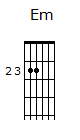
\includegraphics[width=3cm]{../Akordy/em.png}
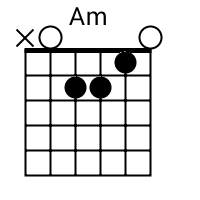
\includegraphics[width=3cm]{../Akordy/am.png}
\end{figure}
\newpage
\addcontentsline{toc}{section}{Hlídač krav}\input{../songy/Hlidackrav}\newpage
\addcontentsline{toc}{section}{Je jaká je}\input{../songy/Jejakaje}\newpage
\addcontentsline{toc}{section}{Kamarádi}%\documentclass[../main.tex]{subfiles}

\begin{song}{title=\centering Kamarádi \\\normalsize Poslední výstřel  \vspace*{-0.3cm}}  %% sem se napíše jméno songu a autor
\moveright \stred \vbox{      %Varianta č. 1  ---> Jeden sloupec zarovnaný na střed


\sloka
	^{Emi}Bývaly chvíle, kdy jsem ^{G}chtěl  sundat 
 
	brýle a ^{Ami}říct ti: ,,Pojď ^{C}ven.``

	Pak jsem to ale nějak překousl, 

	ač jsi mě rozhněval hodně.

\sloka
	Bývaly chvíle, kdy mi nebylo milé, 

	že patřím k takovým lidem. 

	Ne, ne, kámoše si nevybereš, 

	kámoš je ten, kdo na tebe zbyde.

\refren
	Pořád jsme kamarádi, pořád jsme kamarádi.

	Pořád jsme kamarádi, pořád jsme kamarádi.

	Co jsme si, to jsme si, co jsme si, to jsme si 

	pořád jsme kamarádi.

	Co jsme si, to jsme si, co jsme si, to jsme si,

	pořád jsme kamarádi.

\sloka
	Bývaly chvíle, kdy sis chtěl sundat 

	brýle a říct mi: \uv{Pojď ven}. 

	Pak jsi to ale nějak překousl,

	ač jsem tě rozhněval notně.

\sloka
	Bývaly chvíle kdy ti nebylo milé,

	že patříš k takovým lidem.

	Kámoše si prostě nevybereš,

	kámoš je ten kdo na tebe zbyde.

\refren

}
\setcounter{Slokočet}{0}

\end{song}

\newpage %není hotovo
\addcontentsline{toc}{section}{Karavana mraků}\input{../songy/Karavanamraku}\newpage	
\addcontentsline{toc}{section}{Knocking On Heaven's Door}%\documentclass[../main.tex]{subfiles}


\begin{song}{title=\centering Knockin' On Heaven's Door \\\normalsize Bob Dylan  \vspace*{-0.3cm}}  %% sem se napíše jméno songu a autor
\moveright 4.5cm \vbox{      %Varianta č. 1  ---> Jeden sloupec zarovnaný na střed

\sloka
	^{G}Mama, ^{D}take this badge off of me ^{Ami} 
 
	^{G}I can't ^{D}use it ^{C}anymore. 
 
	It's gettin' dark, too dark for me to see.

	I feel like I'm knockin' on heaven's door.

\refren
	^{G}Knock, knock, ^{D}knockin' on heaven's  ^{Ami}door.

	^{G}Knock, knock, ^{D}knockin' on heaven's  ^{C}door. 
 
	Knock, knock, knockin' on heaven's door.

	Knock, knock, knockin' on heaven's door.

\sloka
	Mama, put my guns in the ground 

	I can't shoot them anymore. 

	That long black cloud is comin' down. 

	I feel like I'm knockin' on heaven's door. 

\refren

}
\setcounter{Slokočet}{0}
\end{song}
\begin{figure}[h]
\centering
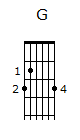
\includegraphics[width=3cm]{../Akordy/g}
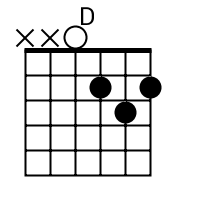
\includegraphics[width=3cm]{../Akordy/d}
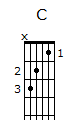
\includegraphics[width=3cm]{../Akordy/c}
\includegraphics[width=3cm]{../Akordy/Am}
\end{figure}
\newpage
\addcontentsline{toc}{section}{Kutil}%\documentclass[../main.tex]{subfiles}

\begin{song}{title=\centering Kutil \\\normalsize Chinaski  \vspace*{-0.3cm}}  %% sem se napíše jméno songu a autor
\moveright 5cm \vbox{      %Varianta č. 1  ---> Jeden sloupec zarovnaný na stře

\sloka
Jsem ^{E}kutil. 

Mám malou ^{F#mi}dílnu víc mě ^{A{\color{white}\_\_}E}nezajímá, 

mé ^{E{\color{white}\_}}hobby je moje práce, 

šťastnej ^{F#mi}člověk každej ^{A}kdo to ^{{\color{white}\_}E}tak má. 

Mám ^{E}ženu. 

Je mladá ^{F#mi}krásná chytrá ^{A{\color{white}\_\_}E}přívětivá. 

Má jednu malinkatou ^{E{\color{white}\_}}chybu, 

že si ^{F#mi}se mnou vůbec ^{A{\color{white}\_\_}E}nepovídá.

\refren
A tak ^{F#mi}hledám holku sdílnou, 

co by chtěla kluka s dílnou, 

^{A}abych nebyl ^{H}sám. ^{H7} 

\textbf{E  F#mi  A  E  C#mi  A  G  D  E } 

\sloka
Jsem kutil. 

Mám malou dílnu víc mě nezajímá. 

Má práce je moje hobby, 

šťastnej člověk každej kdo to tak má. 

Mám ženu. 

Je mladá krásná chytrá přívětivá. 

Má jednu malinkatou chybu, 

že si se mnou vůbec nepovídá.

\refren

}
\setcounter{Slokočet}{0}
\end{song}
\newpage
\addcontentsline{toc}{section}{Lano co k nebi nás poutá}\input{../songy/Lanocoknebinaspouta}\newpage
\addcontentsline{toc}{section}{Leaving On A Jet Plane}\documentclass[../main.tex]{subfiles}

\chapter{Leaving on a jet plane}

\noindent \begin{minipage}{0.5\linewidth}
\begin{song}{title=Leaving on a jet plane}
\begin{verse}
All my bags^{C} are packed I'm ready^{F} to go\\
I'm standing^{C} here outside^{F} your door\\
I hate^{C} to wake you up^{F} to say goodbye^{G7} \\
But the dawn^{C} is breaking it's early^{F} morn\\
The taxi's^{C} waitin' he's blownin'^{F} his horn\\
Already^{C} I'm so lonesome^{F} I could die^{G7}\\
\end{verse}
\begin{verse*}
\hspace*{-0.45cm}\textbf{R:}So kiss^{C} me and smile^{F} for me\\
Tell^{C} me that you'll wait^{F} for me\\
Hold^{C} me like you'll never^{F} let me go^{G7} \\
Cause I'm^{C} leavin' on^{F} a jet plane\\
Don't^{C} know when I'll^{F} be back again\\
Oh,^{C} babe^{F}  I hate to go^{G7}\\
\end{verse*}
\begin{verse}
There's is many^{C} times I've let^{F} you down\\
So many^{C} time I've played^{F} around\\
I tell^{C} you now they^{F} don't mean a thing^{G7} \\
Every place^{C} I go I'll think^{F} of you \\
Every song^{C} I sing I'll sing^{F} for you \\
When I^{C} come back I'll bring^{F} your wedding ring^{G7} \\
\end{verse}
\end{song}
\end{minipage}
\begin{minipage}{0.5\textwidth}
\vspace*{-9.5cm}
\begin{song}{title=Leaving on a jet plane}
\begin{verse*}
\hspace*{-0.45cm}\textbf{R:}So kiss^{C}$\dots$
\end{verse*}
\begin{verse}
\item[3.]Now^{C} the time come^{F} to leave you \\
One^{C} more time let^{F} me kiss you \\ 
Then^{C} close your eyes I'll^{F} be on my way^{G7} \\
Dream^{C} about the days^{F} to come \\
When I^{C} won't have to leave^{F} alone \\
About the times I^{F} won't have to say^{G7} \\
\end{verse}
\begin{verse*}
\hspace*{-0.45cm}\textbf{R:}So kiss^{C}... \\
\end{verse*}
\end{song}
\end{minipage}\newpage
\addcontentsline{toc}{section}{Lemon Tree}%\documentclass[../main.tex]{subfiles}

\begin{song}{title=\centering Lemon Tree \\\normalsize Fool's Garden  \vspace*{-0.3cm}}  %% sem se napíše jméno songu a autor
\moveright 1cm \vbox{      %Varianta č. 1  ---> Jeden sloupec zarovnaný na střed	
\begin{minipage}[t]{0.48\textwidth}\setlength{\parindent}{0.45cm}  %Varianta č. 2 --> Dva sloupce

\sloka
I'm ^{Emi{\color{white}\_}}sittin' here in the ^{Hmi}boring room,

It's ^{Emi}just another rainy Sunday ^{Hmi}afternoon.

I'm ^{Emi{\color{white}\_\_}}wasting my time I got ^{Hmi}nothing to do,

I'm ^{Emi{\color{white}\_}}hangin' aroud I got ^{Hmi}waitin' for you.

But ^{Ami{\color{white}\_\_}}nothing ever happens^{H}

And I ^{Emi{\color{white}\_\_}}wonder.

\sloka
I'm drivin' aroud in my car,

I'm drivin' too fast, I'm drivin' too far,

I'd like to change my point of view,

I feel so lonely I'm waiting for you.

But nothing ever happens.

\refren
^{G}I wonder how, ^{D\,\,\,\,\,\,\,\,\,}wonder why

^{Emi{\color{white}\_\_}\,\,}Yesterday you told me 'bout the ^{Hmi}blue

 ^{\phantom{.}}blue sky

And ^{C}all that I can ^{D}see

Is just a yellow ^{G\,\,\,\,\,\,}lemon tree.^{D} 

I'm ^{G{\color{white}\_\_}}turnin' my head ^{D}up and down.

^{Emi}I'm turnin', turnin', turnin', ^{Hmi}turnin',

 ^{\phantom{.}}turnin' around

And ^{C}all that I can ^{D}see

Is just a yellow ^{G{\color{white}\_\_}}lemon tree.^{D} 

\sloka
^{4(Emi Hmi) Ami H Emi}Sing\,dip,\,ta\,da\,da\,dap\,di\,dap\,dam\elipsa.\elipsa.\elipsa.

\end{minipage}\begin{minipage}[t]{0.48\textwidth}\setlength{\parindent}{0.45cm}  % V případě varianty č.2 jde odsud text do pravé části
\vspace*{0.58cm}
\sloka
I'm sittin' here, I miss the power,

I'd like to go out, takin' a shower.

But there's a heavy cloud inside my head,

I feel so tired put myself into bed

Where nothing ever happens

And I wonder.

\sloka
^{H{\color{white}\_\_\_}}Isolation ^{Emi}is not good for me.

^{D{\color{white}\_\_\_}}Isolation, ^{G}I don't want to

^{H}sit on a lemon tree.

\sloka
I'm steppin' around in a desert of joy,

Baby, anyhow I get another toy

And everything will happen

And you'll wonder.

\refren
%^{G}I wonder how\elipsa\dots \\

\refren
%^{G}I wonder how\elipsa\dots \\


\dots\,and all that I can see --

and all that I can see --

and all that I can see 

Is just a yellow lemon tree.

\end{minipage}
}
\setcounter{Slokočet}{0}
\end{song}\newpage
\addcontentsline{toc}{section}{Made in Valmez}%\documentclass[../main.tex]{subfiles}

\begin{song}{title=\centering Made in Valmez \\\normalsize Mňága a Žďorp  \vspace*{-0.3cm}}  %% sem se napíše jméno songu a autor
\moveright 4cm \vbox{      %Varianta č. 1  ---> Jeden sloupec zarovnaný na střed	

\sloka
^{A{\color{white}\_}}Jako je sama skála, ^{D}tak jsem sám i ^{Hmi}já. ^{E} 

Jako je prázdná duha, tak jsem prázdný i já. 

Jako je zrádná voda, tak zradím i já. 

\refren
^{A{\color{white}\_\_\_\_\_}}Zkouším se prokopat ven -- zkouší se prokopat ven! 

^{D{\color{white}\_\_\_\_\_}}Zkouším se prokopat ven -- ^{Hmi{\color{white}\_}}zkouší se ^{A{\color{white}\_\_\_}}prokopat ven! 

^{A{\color{white}\_\_\_\_\_}}Zkouším se prokopat ven -- zkouší se prokopat ven! 

^{D{\color{white}\_\_\_\_\_}}Zkouším se prokopat ven! ^{Hmi\,\,\,A} 

\sloka
O půl třetí na náměstí ve Valašském Meziříčí 

jdu co noha nohu mine a každý sám sobě jsme stínem. 


\sloka
Nic mi není přitom melu z posledního, 

těžko říct o tom něco konkrétního. 

Stejná slova kolem stejný tváře 

a každý sám sobě jsme lhářem a já už zase. 

\refren

\refren

}
\setcounter{Slokočet}{0}
\end{song}
\newpage
\addcontentsline{toc}{section}{Milionář}%\documentclass[../main.tex]{subfiles}

\begin{song}{title=\centering Milionář \\\normalsize Jaromír Nohavica  \vspace*{-0.3cm}}  %% sem se napíše jméno songu a autor
\moveright 1cm \vbox{      %Varianta č. 1  ---> Jeden sloupec zarovnaný na střed	
\begin{minipage}[t]{0.48\textwidth}\setlength{\parindent}{0.45cm}  %Varianta č. 2 --> Dva sloupce

\sloka
^{D}U nás v domě ^{A}říkají mi Franta ^{D}Šiška

bo už od pohledu ^{G}chytry jsem jak ^{D}liška 

a dyž ^{A}kery něco neví 

nebo ^{D}dyž je na co levy  

tak de za ^{Emi}mnu a ja ^{A}všecko najdu v ^{D}knižkach 

\sloka
Raz mi říkal jeden znamy dole v baře 

že s tu hlavu moh bych do Milionaře 

čemu ne říkám si brachu 

šak má Železný dost prachu 

no a Čechovi se podíváš do tvaře 

\sloka
Dostal jsem se mezi partu uchazeču 

nikdo nemá šajnu jak tam nervy teču 

všecko viděl jsem do hnědě

tak jsem zmáčknul AbeCeDe 

no a už mě kruci ke stolečku vleču 

\sloka
Čech to začal takym malym interviju 

co pry robim esi kuřim a co piju 

tak jsem řeknul co jsem řeknul 

on se evidentně leknul 

a už začly blikat světla ve studiu

\sloka
to se přiznam nebylo mi vesele

První otázka pry co je ukulele 

tož tak jsem radši hlavu sklonil 

abych to všecko nezkonil 

říkám chtěl bych se obratit na přitele

\sloka
Lojza byl po hlasu silně nevyspaly 

asi zase celu šichtu prochlastali 

bylo slyšet jak tam dycha 

ale třicet vteřin ticha 

to je tak dyž se vam kamarad navali.

\sloka
Moju staru zatím doma braly mory 

lidi ohryzavali televizory 

tož padesat na padesat 

ať vím esi su to ty bulharské hory

\end{minipage}\begin{minipage}[t]{0.48\textwidth}\setlength{\parindent}{0.45cm}\vspace*{0.55cm}  % V případě varianty č.2 jde odsud text do pravé části


\sloka
A už jasně na tym komputuře sviti 

buďto je to za A vzacne lučni kviti 

nebo za Be nastroj strunny 

tu de kurňa o koruny 

a ja stejně jak na začatku jsem v řiti 

\sloka
Čech tam zatím maval tymi svymi čisly

tak si řikam Franta napij sa a mysli 

jake tudy sakypaky 

obratiš se na divaky

šak tu zatím za ty prachy enem kysli 

\sloka
Sam jsem byl zvědavy co publikum zvoli 

bo aj v obecenstvu možu sedět voli 

devadesat procent za Be 

ale to mi přišlo slabe 

bo co není stopro to mě dycky smali 

\sloka
Ještě že jsem chlap co zboja neutika 

říkam pane Čechu pujdem do rizika 

měl jsem v gaťach nadělano 

ale Čech zakřičel ano 

mate pravdu je to nastroj hudebnika

\sloka 
Lidi tleskali bo uspech to byl plny 

radosti zrobili dvě mexicke vlny 

a ja co mam srdce skromne 

jako všeci z Dolni Lomne 

jsem byl spokojeny bo sem ukol splnil 

\sloka
Pane Čechu nerad přetahnul bych strunu 

končim hru a beru tisicikorunu 

Čech se jenom chytnul stolu 

obočí mu spadlo dolu 

no a už se modry ku podlaze sunul 

\sloka
První třidu do Ostravy Intercity 

v jidelňaku celu cestu valim kyty 

a ta stovka co mi zbude 

to je přispěvek na chude 

bo Ostrava je region razovity.


\end{minipage}
}
\setcounter{Slokočet}{0}
\end{song}\newpage
\addcontentsline{toc}{section}{Nagasaki Hirošima}\begin{song}{title=\predtitle\centering Nagasaki Hirošima \\\large Mňága \&  Žďorp  \vspace*{-0.3cm}}  %% sem se napíše jméno songu a autor
\begin{centerjustified}
\nejnejvetsi

\sloka
	^{A\z }Tramvají ^{E\z }dvojkou ^{D\z }jezdíval ^{E}jsem do ^*{\z A}Žideni c, ^{E\,\,D\,\,E}

	z ^{A}tak velký ^{E\z }lásky ^{D\z}většinou ^{E\z }nezbyde ^{F#mi\z }nic.~~~

	Z ^{D\z }takový ^{A\z}lásky ^{D\z}jsou kruhy ^{A\z}pod ^{{\color{white}\_}E}očima

	a dvě ^*{A}sp álený ^{E\z }srdce -- ^{D\z }Nagasaki ^{E\z}Hirošima. ^{A\,\,E\,\,D\,\,E}

\sloka
	Jsou jistý věci, co bych tesal do kamene,
	
	tam, kde je láska, tam je všechno dovolené
	
	a tam, kde není, tam mě to nezajímá.
	
	Jó dvě spálený srdce Nagasaki Hirošima.

\sloka
	Já nejsem svatej, ani ty nejsi svatá,
	
	jablka z ráje bejvala jedovatá,
	
	jenže hezky jsi hřála, když mi někdy byla zima.
	
	Jó dvě spálený srdce Nagasaki Hirošima.

\sloka
	Tramvají dvojkou jezdíval jsem do Židenic,
	
	z takový lásky většinou nezbyde nic.
	
	Z takový lásky jsou kruhy pod očima

	/: a dvě spálený srdce Nagasaki Hirošma. :/
	
	/: A dvě spálený srdce Nagasaki Hirošma. :/

\end{centerjustified}
\setcounter{Slokočet}{0}
\end{song}


\begin{figure}[h]
\predtitle\centering
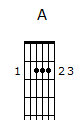
\includegraphics[width=3cm]{../Akordy/a.png}
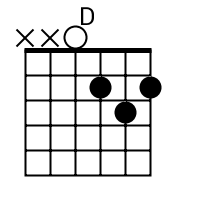
\includegraphics[width=3cm]{../Akordy/d.png}
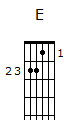
\includegraphics[width=3cm]{../Akordy/e.png}
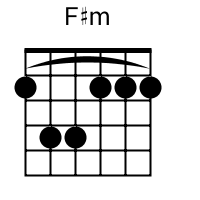
\includegraphics[width=3cm]{../Akordy/fxm.png}
\end{figure}
\newpage
\addcontentsline{toc}{section}{Orlice}\documentclass[../main.tex]{subfiles}

\chapter{Orlice}

\noindent
\begin{minipage}{0.5\linewidth}
\begin{song}{title=Orlice}


\begin{verse}[numbered]
	^{A}Orlice zas ^{E}šumí nad spla^{F#mi}vem \\
	Dodpusť mi ^{A}modlím se ať ^{E}všechno přesta^{C#mi}nem' \\
	odpusť mi ^{D}ke smutku ten ^{E}chlad \\
	je květen a ne listo^{F#mi}pad \\
	odpusť ^{A}modlím se když ^{E}spáváš na pra^{D}vém boku \\
\end{verse}

\begin{verse}[numbered]
	Když Orlice zas šumí nad splavem \\
	odpusť mi modlím se ať všechno přestanem' \\
	odpusť, že nemám na duši \\
	smutek ač králi Artuši \\
	prý utek' kůň i s bílým praporem\\
\end{verse}

\begin{verse}[numbered]
	^{C/G}Vysoko ^{G}v horách prší ^{A/E}kolem přelít ^{D}hvízdák \\
	Vysoko v horách prší na pyruších hnízda \\
	Vysoko v horách prší Dáša ruší, hvízdá \\
	Vysoko v horách horko v autobuse bonbon v puse ^{H}a ty hvízdáš s^{E} ní zdaleka \\
\end{verse}

\begin{verse}[numbered]
	Orlice zas šumí nad splavem \\
	odpusť mi modlím se ať všechno přestanem' \\
	odpusť ať nemám nikdy strach \\
	kéž dýchám na zobáčcích vah \\
	odpusť Orlice zas šumí nad splavem \\
\end{verse}

\end{song}
\end{minipage}
\begin{minipage}{0.5\textwidth}
\vspace*{-3.3cm}
\begin{song}{title=Orlice}
\begin{verse}
\item[5.]Vysoko v horách prší voda na tři couly\\ 
	Vysoko v horách prší Dáša už se choulí \\
	Vysoko v horách prší na kalhotách bouli \\
	Vysoko v horách horko v autobuse sucho v puse co si počneš s ní zdaleka \\
\end{verse}
\begin{verse}
\item[6.]Orlice zas šumí nad splavem \\
	odpusť mi modlím se ať všechno přestanem' \\
	odpusť, že nemám na duši smutek ač králi Artuši \\
	prý utek' kůň i s bílím praporem \\
\end{verse}
\begin{verse}
\item[7.]sólo
\end{verse}	
\begin{verse}
\item[8.]Orlice zas šumí nad splavem \\
	odpusť mi modlím se ať všechno přestanem' \\
	odpusť ať nemám vůbec strach \\
	kéž dýchám na zobáčcích vah \\
	odpusť Orlice zas šumí nad splavem\\
\end{verse}
\end{song}
\end{minipage}
\newpage
\addcontentsline{toc}{section}{Ostravo}%\documentclass[../main.tex]{subfiles}

\begin{song}{title=\centering Ostravo \\\normalsize Jaromír Nohavica  \vspace*{-0.3cm}}  %% sem se napíše jméno songu a autor
\moveright \stred \vbox{      %Varianta č. 1  ---> Jeden sloupec zarovnaný na střed	

\refren
^{Dmi}Ostravo, Ostra^{A7}vo,

město mezi městy, ^{Dmi}hořké ^{A7}moje štěstí.

^{Dmi}Ostravo, Ostra^{A7}vo, 

černá hvězdo nad hla^{Dmi}vou.

\sloka
^{C}Pán Bůh rozdal jiným ^{F}městům všecku krásu, 

^{Gmi}parníky na řekách a ^{A7}dámy všité do atlasu. 

^{Dmi}Ostravo -- srdce ru^{A7}dé,

zpečetěný osu^{Dmi}ide. ^{A7}  ^{Dmi}

\refren

\sloka
Ať mě moje nohy nesly, kam mě nesly, 

ptáci na obloze jenom jednu cestu kreslí.

Ostravo - srdce rudé,

zpečetěný osude.

}
\setcounter{Slokočet}{0}
\end{song}
\newpage
\addcontentsline{toc}{section}{Pangajó}%\documentclass[../main.tex]{subfiles}

\begin{song}{title=\centering Pangajó \\\normalsize \vspace*{-0.3cm}}  %% sem se napíše jméno songu a autor
\moveright 6cm \vbox{      %Varianta č. 1  ---> Jeden sloupec zarovnaný na střed	

\sloka
^{Ami}Pangajo, Pangajo
 
^{Dmi}ka mudi ^{Ami}ka

rodi ^{G}he rodi hu 

arong ^{Ami}baina ^{G}pondi ^{Ami}he  

te hu ^{G}a kema ^{Ami}o  

Te hu ^{G}a kema ^{Ami}o aó aó aó 

}
\setcounter{Slokočet}{0}
\end{song}
\newpage
\addcontentsline{toc}{section}{Písnička pro Tebe}\begin{song}{title=\predtitle\centering Písnička pro Tebe \\\large Mňága a Žďorp  \vspace*{-0.3cm}}  %% sem se napíše jméno songu a autor
\begin{centerjustified}
\nejnejvetsi

\sloka
^{F\,}To je ta ^{C{\color{white}\_\_}G{\color{white}\_}}písnička pro te^{C\,}be 

^{F}z ^{C{\color{white}\_\_}\,\,G\,C}autobusáku,

^{{\color{white}\_\_}\,\,F}mrazivé ^{C}a modravé ^{G{\color{white}\_\_}}obrysy ^{C{\color{white}\_\_}}mraků 

^{F\,\,\,C\,\,}ptáků a ^{{\color{white}\_\_}G\,C}paneláků. 

\sloka
Nic není, co by stálo aspoň za něco 

a něco nestojí ani za to. 

Nic není, co by stálo aspoň za něco 

a něco nestojí ani za to. 

\sloka
Co za to stojí, to neví nikdo. 

Někdo možná snad, ale nikdo neví kdo. 

Co za to stojí, to neví nikdo. Nikdo. 

To je ta písnička pro tebe. 

\sloka = 1.

\sloka
/:Pro tebe\elipsa\dots\,:/ 

/:Pro tebe\elipsa\dots\,:/ 

/:Pro tebe\elipsa\dots\,:/ 

Pro tebe\elipsa\dots

\end{centerjustified}
\setcounter{Slokočet}{0}
\end{song}
\newpage
\addcontentsline{toc}{section}{Podzimní}\begin{song}{title=\predtitle\centering Podzimní \\\large Karel Plíhal  \vspace*{-0.3cm}}  %% sem se napíše jméno songu a autor
\begin{centerjustified}
\nejvetsi

\sloka
^*{A}Po dzimní obloha dala se ^{D}do gala, 

^*{E}ve černí vánek se do vlasů ^{A{\color{white}\_\_}}vplétá, 

a po tý obloze na křídle ^{D{\color{white}\_\_}}rogala 

s ^{E\,\,}tím vánkem ve vlasech Markéta ^{A{\color{white}\_}}létá.

\sloka
Nebe je modrý jako mý džíny, 

tak jsme si zpívali s klukama zamlada, 

zmizely smutky a podzimní splíny, 

prostě to všechno, co Markéta nerada. 

\sloka
Vysoko na nebe, hluboko do polí 

Markéta létá a přitom si zpívá, 

co oči nevidí, to srdce nebolí, 

je totiž podzim a brzo se stmívá. 

\sloka
Zmizely splíny a přívaly pláče 

a s nima ty protivný přízraky z minula,

připravte obvazy, dlahy a fáče, 

kdyby se náhodou se zemí minula. 

\sloka = 1.

\sloka = 2.

\sloka = 3.

\sloka = 4.

\sloka
/: Podzimní obloha dala se do gala, 

večerní vánek se do vlasů vplétá. :/ 

 Podzimní obloha dala se do gala, 
 
večerní vánek se do vlasů vplétá.

\end{centerjustified}
\setcounter{Slokočet}{0}
\end{song}
\newpage
\addcontentsline{toc}{section}{Převrat v Banánové republice} \documentclass[../main.tex]{subfiles}

\chapter{Převrat V Banánové Republice\\ \scalebox{0.8}[0.8]{Znouzecnost}}
\noindent\hspace{0.15\linewidth}\begin{minipage}{0.7\linewidth}
\begin{song}{title=Pangajó}

\begin{verse}[numbered]
^{F}Generál ^{C}Sancho ^{B}Grácia ^{C}zmocnil ^{F}se vlády ^{C} ^{B} ^{C} \\
v Banánový republice někde uprostřed pralesa. \\
Hlásili to po ránu ve zprávách a psali v novinách, \\
Banánová republika, kde není nic jinýho než banány ^{F}a ^{C}armáda ^{B} ^{C}
\end{verse}
\begin{verse*}
\hspace*{-0.45cm}\textbf{R:}  ^{Dmi}A já vám ^{B} řikam, že ^{C}z tohodle nekouká ^{F} zas nic ^{C} dobrý ^{Dmi} ho \\
^{Dmi}A já vám ^{B} říkam že ^{C} banány teď budou ^{F} zas o něco ^{C} dražší, ^{F}zas o něco ^{C}dražší ^{F} zas o něco ^{C} dražší^{B} ou ^{F}jééé.
\end{verse*}
\begin{verse}[numbered]
Generál Sancho Grácia stojí na balkóně \\
a hází po lidech slibama že bude líp. \\
A lidi vyskakují a lidi jsou rádi, \\
ale byli by radši, kdyby po nich házel koláče a řízky. \\
\end{verse}
\begin{verse*}
\hspace*{-0.45cm}\textbf{R:} 
\end{verse*}
\begin{verse}[numbered]
V Banánový republice je dneska hrozně veselo, \\
generála Sancha Gráciu hodili lidi z balkónu \\
a sním jeho poskoky a patolízaly, \\
a armáda složila zbrane, no to je veselo, veselo, veselo!
\end{verse}
\begin{verse*}
\hspace*{-0.45cm}\textbf{R:} 
\textbf{G  D  C  D}
\end{verse*}
\begin{verse}[numbered]
Dámy pánové, tá svržena vláda sedí momentálně v hostinci U exilu \\
a nalejvá si hlavy banánovým vínem a přemýšlí, \\
přemýšlí jak se dostat zpátky k moci.\\
No, když bude dost dlouho přemejšlet, tak určitě na něco přijde,\\
co třeba takhle vojensko-politický převrat!\\
\end{verse}
\end{song}
\end{minipage}\newpage
\addcontentsline{toc}{section}{Ráda se miluje}%\documentclass[../main.tex]{subfiles}

\begin{song}{title=\centering Ráda se miluje \\\normalsize Karel Plíhal  \vspace*{-0.3cm}}  %% sem se napíše jméno songu a autor
\moveright 4cm \vbox{      %Varianta č. 1  ---> Jeden sloupec zarovnaný na střed	

\refren
^{Hmi}Ráda se miluje, ^{A{\color{white}\_}}ráda ^{D}jí,

^{G{\color{white}\_}}ráda si ^{F#mi\,}jenom tak ^{Hmi{\color{white}\_}}zpívá, 

vrabci se na plotě ^{A\,{\color{white}\_}D\,}hádají, 

^{G{\color{white}\_\_}}kolik že ^{F#mi}času jí ^{Hmi{\color{white}\_}}zbývá.

\sloka
^{G}Než vítr dostrká k ^{D\,{\color{white}\_}}útesu ^{G}tu její legrační ^{{\color{white}\_}D\,\,F#mi}bárku 

a ^{Hmi\,\,}Pámbu si ve svým ^{A{\color{white}\_}D}notesu ^{G{\color{white}\_\_}}udělá ^{F#mi}jen další ^{Hmi\,\,}čárku.

\refren

\sloka
Psáno je v nebeské režii, a to hned na první stránce, 

že naše duše nás přežijí v jinačí tělesný schránce. 

\refren

\sloka
Úplně na konci paseky, tam, kde se ozvěna tříští, 

sedí šnek ve snacku pro šneky -- snad její podoba příští. 


\refren

}
\setcounter{Slokočet}{0}
\end{song}

\newpage
\addcontentsline{toc}{section}{Russian mystic pop IV.}\begin{song}{title=\centering Russian mystic pop IV. \\\normalsize Psí vojáci  \vspace*{-0.3cm}}  %% sem se napíše jméno songu a autor
\moveright 4cm \vbox{      %Varianta č. 1  ---> Jeden sloupec zarovnaný na střed	

\sloka 
	^{Ami{\color{white}\_}}Chodím po tom městě a ^{F{\color{white}\_\_\_}}nemám ani na tramvaj.
	
	^{G{\color{white}\_}}Není jaksi na místě, že ^{Ami}bych se z toho vyhrabal.
	
	^{Ami}Půjčil jsem si pětistovku a ^{F}od výčepu k báru
	
	^{G}jsem ji mezi prstama ^{{\color{white}\_}Ami}proměnil v mlžnou páru.
	
\refren
	/: Hej ^{Ami}hej \dots hej ^{F}hej \dots hej ^{G}hej \dots jsem ^{{\color{white}\_\_}Ami}mladej. :/
	
	 /:^{Gmi{\color{white}\_}}Připadá mi to děsný ale ^{D{\color{white}\_\_}}začíná mi bejt ^{F{\color{white}\_}}tohle město ^{C{\color{white}\_}}těsný. :/
	 
 	 ^{Gmi{\color{white}\_}}Připadá mi to děsný ale ^{D{\color{white}\_\_}}začíná mi bejt ^{F{\color{white}\_}}tohle město ^{C{\color{white}\_}}těsný. 

\sloka
	Ani šanci nemám, že bych se ráno nasnídal,
	
	příteli se ozvu na oběd se pozvu.
	
	Z hlediska věčnosti jsem plnej blbostí,
	
	subspecie ternitatis holky, holky -- Dakar Paris.

\refren

\sloka
	Až večer budu usínat, schoulím se do sebe
	
	a budu vzpomínat že měl jsem kdysi tebe.
	
	Nikdo už mi nezavolá nikdo už mě nepohladí,
	
	všem lidem totiž moje bytost vadí.

\refren

}
\setcounter{Slokočet}{0}
\end{song}\newpage
\addcontentsline{toc}{section}{Sametová}\begin{song}{title=\centering Sametová \\\normalsize Žlutý pes  \vspace*{-0.3cm}}  %% sem se napíše jméno songu a autor
\moveright 4.5cm \vbox{      %Varianta č. 1  ---> Jeden sloupec zarovnaný na střed	

\sloka 
	^{G}Vzpomínám, když tehdá ^{C}před léty ^{G}začaly lítat ^{C}rakety,

	^{G}zdál se to bejt ^{C}docela dobrej ^{D}nápad,

	^{G}saxofony hrály ^{C}unyle, ^{C}frčely švédský ^{C}košile

	^{G}a někdo se moh' ^{Emi}docela dobře ^{C}flákat. ^{D}
	
\sloka
	 Když tam stál rohatej u školy, my neměli podepsaný úkoly,

	už tenkrát rozhazoval svoje sítě,

	poučen z předchozích nezdarů sestrojil elektrickou kytaru  
	
	a rock'n'roll byl zrovna narozený dítě.
	
\refren
	^{G}Vzpomínáš, takys' tu ^{D}žila, a ^{Emi}nedělej, že si ^{C}jiná,

	taková ^{G}malá pilná ^{D}včela, taková ^{C}celá ^{D}\ldots \, ^{G}sametová.
	
	
\sloka
	Přišel čas a jako náhoda byla tu bigbítová pohoda,
	
	kytičky a úsmevy sekretárok,
	
	sousedovic bejby Milena je celá blbá z Boba Dylana,
	
	ale to nevadí, já mám taky nárok.

\sloka
	Starý, mladý nebo pitomí mlátili do toho jako my,
	
	hlavu plnou Londýna nad Temží,
	
	a starej dobrej satanáš hraje u nás v hospodě mariáš
	
	a pazoura se mu trumfama jenom hemží.

\refren
	Vzpomínáš, už je to jinak, a jde z toho na mě zima,
	
	ty jsi, holka, tehdá byla taková celá \dots \,sametová.
	
\sloka
	A do toho tenhle Gorbačov, co ho znal celej Dlabačov,
	
	kopyta měl jako z Arizony,
	
	přišel a zase odešel a nikdo se kvůli tomu nevěšel
	
	a po něm tu zbyly samý volný zóny.

\refren
	Vzpomínáš, jak jsi se měla, když jsi nic nevěděla,
	
	byla to taková krásná cela a byla celá \dots
	 
	Vzpomínáš, jak jsi se měla, když jsi nic nevěděla,
	
	byla to taková krásná cela a byla celá \dots \,sametová.

}
\setcounter{Slokočet}{0}
\end{song}


\newpage
\addcontentsline{toc}{section}{Slaboch Ben}\begin{song}{title=\centering Slaboch Ben \\\normalsize Kapitán Kid  \vspace*{-0.3cm}}  %% sem se napíše jméno songu a autor
\moveright 0.8cm \vbox{      %Varianta č. 1  ---> Jeden sloupec zarovnaný na střed	
\begin{minipage}[t]{0.48\textwidth}\setlength{\parindent}{0.45cm}  %Varianta č. 2 --> Dva sloupce

\sloka 
	^{C}V lesích ^{Ami}Ontaria ^{F}čerstvá smůla ^{G}voní.

	^{C}Tam, kde silných ^{A7}mužů paže ^{Dmi}vládne ^{G}jen,

	kde ^{C}sosny ^{Ami}staleté se ^{F}pod sekyrou ^{Cdim}kloní,

	v kempu ^{C}dřevorubců ^{G7}žije Slaboch ^{C}Ben.
	
\sloka
^{F}Mlčí stále ^{Cdim}jen a ^{C}snáší strasti ^{Ami}žití

a když ^{Dmi}kamarádů ^{G7}výsměch dávno ^{Ami}ztich.

^{E}V noci nad ^{Ami}jezerem, ^{Dmi}Polárka když ^{Ami}svítí,

^{E}odpouští jim věčný jejich smích.

\refren
	^{A}Že je slaboch, ^{A7}že prý nemá

	^{D}sílu, že se vrány bojí,

	^{E}říká o něm ^{E7}předák Andy ^{A}Renn.

	(Ten kojot) Hodí se jen ^{A7}k tomu, aby

	^{D}chodil kempu ^{D7}pro zásoby,

	^{E}je prý jenom ^{E7}pro smích Slaboch ^{A}Ben. ^{G7}

\sloka
	Na cestu mu dává bez nábojů zbraně,
	
	kdyby se snad před kojoty bránit chtěl.
	
	Kdyby se mu chtělo vystřelit si na ně,
	
	že by stejně, jak se míří nevěděl.
	
	Bez nábojů prý se aspoň nepostřelí,
	
	kdyby třeba přemoh strach a ránu dal.
	
	A když ještě dodal: "Snad se vrátíš celý,"
	
	kemp se málem smíchy rozsypal.
	
\refren
\end{minipage}\begin{minipage}[t]{0.48\textwidth}\setlength{\parindent}{0.45cm}\vspace*{0.59cm}  % V případě varianty č.2 jde odsud text do pravé části

\sloka
	Byli by se smáli ještě hodnou chvíli,
	
	kdyby tábor nebyl náhle přepaden
	
	bandou, kterou vedl jednooký Billy,
	
	kterým mnohý traper byl už zastřelen.
	
	Na pět kamarádů deset koltů cílí,
	
	každý z nich už s životem se rozžehnal.

	Když tu náhle výkřik zazní v pravou chvíli:
	
	\uv{Kdo se nevzdá, žít nebude dál!}
	
\refren
	To že je slaboch? Ten že nemá
	
	sílu, že se rány bojí,
	
	říká si teď v duchu Andy Renn.
	
	(Ten kojot) Ten že se nám hodí k tomu,
	
	aby chodil pro zásoby,
	
	tohle přece není slaboch Ben.

\sloka
	Deset koltů nato cíl svůj ihned mění,
	
	míří tam, kde v jejich zádech stojí Ben.

	Leč pět kamarádů v tomtéž okamžení
	
	střelbu spustí, dokud Bill je překvapen.
	
	Pak už v trávě leží jednooký Billy
	
	a s ním jeho čtyři muži mrtvi jen.
	
	Jako šestý s nimi s nenabitou zbraní,
	
	pro své pardy zemřel Slaboch Ben.

\refren
	Že je slaboch, že prý nemá
	
	sílu, že se vrány bojí,
	
	říkal o něm kdysi Andy Renn.
	
	Na hrobě, jenž teď ho kryje
	
	nápis je, že proto žije
	
	pardů pět, že zemřel pro ně Ben.
\end{minipage}
}
\setcounter{Slokočet}{0}
\end{song}

\newpage
\addcontentsline{toc}{section}{Slavíci z Madridu}%\documentclass[../main.tex]{subfiles}

\begin{song}{title=\centering Slavíci z Madridu \\\normalsize Waldemar Matuška \vspace*{-0.3cm}}  %% sem se napíše jméno songu a autor
\moveright 4.5cm \vbox{      %Varianta č. 1  ---> Jeden sloupec zarovnaný na střed	

\sloka
^{Ami}Nebe je ^{E}modrý a zlatý, ^{Ami}bílá sluneční záře,

horko a ^{E}sváteční šaty, ^{Ami}vřava a zpocený tváře,

vím, co ^{E}se bude dít, býk už ^{Ami}se v ohradě vzpíná,

kdo chce, ^{E}ten může jít, já ^{Ami}si dám sklenici vína.

\refren
^{Dmi}Žízeň je ^{Ami}veliká, život mi utíká,

^{E}nechte mě ^{Ami}příjemně snít,

^{Dmi}ve stínu pod ^{Ami}fíky poslouchat slavíky

^{E}zpívat si s ^{Ami}nima a pít.

\sloka
Ženy jsou krásný a cudný, mnohá se ve mně zhlídla,

oči jako dvě studny, vlasy jak havraní křídla,

dobře vím, co znamená pád do nástrah dívčího klína,

někdo má pletky rád, já si dám sklenici vína.

\refren

\sloka
Nebe je modrý a zlatý, ženy krásný a cudný,

mantily, sváteční šaty, oči jako dvě studny,

zmoudřel jsem stranou od lidí, jsem jak ta zahrada stinná,

kdo chce, ať mi závidí, já si dám sklenici vína.

\refren

}
\setcounter{Slokočet}{0}

\end{song}
\begin{figure}[h]
\centering
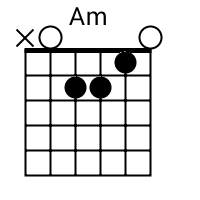
\includegraphics[scale=1.5]{../Akordy/am}
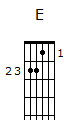
\includegraphics[scale=1.5]{../Akordy/e}
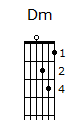
\includegraphics[scale=1.5]{../Akordy/dm}
\end{figure}

\newpage
\addcontentsline{toc}{section}{Sound Of Silence}%\documentclass[../main.tex]{subfiles}

\begin{song}{title=\centering Sound Of Silence \\\normalsize Simon \& Garfunkel  \vspace*{-0.3cm}}  %% sem se napíše jméno songu a autor
\moveright \stred \vbox{      %Varianta č. 1  ---> Jeden sloupec zarovnaný na střed	
\sloka
   ^{Ami}Hello darkness my ^{G}old friend
   
   I've come to talk with you ^{Ami}again
   
   because a ^{C}vision softly ^{F C}creeping
   
   left it seeds while I was ^{F C}sleeping.
   
   And the ^{F}vision that was planted in my ^{C}brain 
   
   still ^{Ami}remains ^{C}within the ^{G}sound of ^{Ami}silence.

\sloka
   In restless dreams I walked alone, 
   
   narrow streets of cobble-stone ,
   
   'neath the halo of a street lamp 
   
   I turned my collar to the cold and damp.
   
   When my eyes were stabbed by the flash of a neon light 
   
   that spilt the night and touched the sound of silence.
   
\sloka
   And in the naked light I saw 
   
   ten thousand people maybe more 
   
   People talking without speaking,
   
   people hearing without listening,
   
   people writing songs that voices never share,
   
   and no one dare disturb the sound of silence.
   
\sloka
   \uv{Fools!} said I \uv{you do not know
   
   silence like a cancer grows 
   
   hear my words that I might teach you 
   
   take my arms that I might reach you.} 
   
   But my words like silent raindrops fell 
   
   and echoed in the wells of silence. 
   
\sloka
   And the people bowed and prayed 
   
   to the neon god they made 
   
   and the sign flashed out its warning 
   
   in the words that it was forming and the sign said: 
   
   \uv{The words of the prophets are written on the subway walls 
   
   and tenament halls} and whisper'd in the sound of silence. 
   

}
\setcounter{Slokočet}{0}
\end{song}
\newpage
\addcontentsline{toc}{section}{Traktor}\begin{song}{title=\predtitle\centering Traktor \\\large Visací zámek \vspace*{-0.3cm}}  %% sem se napíše jméno songu a autor
\begin{centerjustified}

\begin{varwidth}[t]{0.5\textwidth}\setlength{\parindent}{0.45cm}  % V případě varianty č.2 jde odsud text do pravé části

\sloka
^{F\z}Jede ^{\z As\:\:\:\:}traktor,~je~to Zetor,

^{B\z}jede do hor ^{F\z}orat brambor.

\sloka
Zemědělci brambor zasejí,

potom pohnojí, pak zas vyrejí.

Mládenec si kapsu namastí,

prachama zachrastí

na děvu povětrnou.

\refren

/: ^{F{\color{white}\_\_\_}As\,}Kriminalita, ^{F{\color{white}\_\_\_}As\,}kriminalita,
^{F{\color{white}\_\_\_}As\,}kriminalita, 

^{B\z}mládeže. :/

\sloka
Mládenec a děva spolu jdou

před novou hospodou, hrozně se radujou.

Nejdřív se tu spolu opijem,

družstevní prase zabijem

a pak si užijem.

\refren

\sloka
Mládenec se hrozně opije,

vepříka zabije a pak se vzapamatuje.

Svýho čimu ihned lituje,

za mříže putuje

i s děvou povětrnou.

\refren

\sloka
Jede traktor, je to Zetor,

jede do hor orat brambor.

\end{varwidth}\mezisloupci

\end{centerjustified}
\setcounter{Slokočet}{0}
\end{song}
\newpage
\addcontentsline{toc}{section}{Trezor}\begin{song}{title=\centering Trezor \\\normalsize Karel Gott  \vspace*{-0.3cm}}  %% sem se napíše jméno songu a autor
\moveright 3cm \vbox{      %Varianta č. 1  ---> Jeden sloupec zarovnaný na střed	

\sloka 
	^{D}Ze zdi na mě tupě zírá ^{G}po trezoru temná díra,

	^{E7{\color{white}\_\_\_}}poznám tedy bez nesnází, ^{A7}že tam nepochybně něco schází.

	^{D}Ve zdi byl totiž po dědovi ^{G{\color{white}\_}}velký trezor ocelový.

	^{A7{\color{white}\_}}Mám tedy ztrátu zdánlivě ^{{\color{white}\_\_\_}D}minimální.
      
\sloka
	^{D}Na to že ^{A7{\color{white}\_\_\_}}náhodně v krámě vášnivé dámě ^{D{\color{white}\_}}padl jsem za ^{Hmi}trofej,

	^{E7{\color{white}\_\_}}tvrdila pevně: ,,Přijdu tě levně, ^{A7{\color{white}\_\_\_}}nezoufej!`` Ó jé, jé, jé, jé.

	^{D{\color{white}\_\_}}Jenže potom v naší vile ^{G{\color{white}\_\_\_}}chovala se zhůvěřile,

	^{E7}aby měla správné klima, ^{A7}dal jsem ji do trezoru, ať v klidu dřímá.
      
\refren
	^{D{\color{white}\_\_\_}}Spánku se bráním už noc pátou, ^{G}ne ale žalem nad tou ztrátou,

	^{A7}jen hynu bázní, že kasař úlovek ^{G D}vrátí.
      
\sloka = 2.
      
\refren


}
\setcounter{Slokočet}{0}
\end{song}

\newpage
\addcontentsline{toc}{section}{To ta He\v lpa}\begin{song}{title=\centering To ta He\v lpa \\\normalsize  \vspace*{-0.3cm}}  %% sem se napíše jméno songu a autor
\moveright 4cm \vbox{      %Varianta č. 1  ---> Jeden sloupec zarovnaný na střed	

\sloka 
	^{Dmi}To ta ^{G{\color{white}\_\_}}Helpa, ^{Dmi}to ta ^{G{\color{white}\_\_}}Helpa, ^{Dmi\,}to je ^{A7{\color{white}\_\_}}pekné ^{Dmi\,\,}mesto.

	^{Dmi}A v tej ^{G{\color{white}\_\_}}Helpe, ^{Dmi}a v tej ^{G{\color{white}\_\_}}Helpe ^{Dmi\,{\color{white}\_\_}}švarných ^{A7{\color{white}\_\_\_}}chlapcov ^{Dmi}je sto.

	/: ^{B{\color{white}\_\_}}Koho ^{C7}je sto, ^{F\,\,{\color{white}\_}}toho je sto, ^{C}nie po mojej ^{\,\,\,F\,\,A7}vóli,

	^{Dmi}len za ^{G{\color{white}\_\_\_}}jednym, ^{Dmi}len za ^{G{\color{white}\_\_\_}}jednym ^{Dmi\,A7{\color{white}\_\_}}srdiečko ma ^{Dmi}boli. :/


\sloka
	Za Janíčkom, za Palíčkom krok by něspravila,
	
	za Ďuríčkom, za Mišíčkom Dunaj preskočila.

	/: Dunaj, Dunaj, Dunaj, Dunaj, aj to širé pole,
	
	len za jedním, len za jedním, počešenie moje. :/


}
\setcounter{Slokočet}{0}
\end{song}


\newpage
\addcontentsline{toc}{section}{What Makes You Beautiful}%\documentclass[../main.tex]{subfiles}

\begin{song}{title=\centering What Makes You Beautiful \\\normalsize One Direction  \vspace*{-0.3cm}}  %% sem se napíše jméno songu a autor
\moveright 3cm \vbox{      %Varianta č. 1  ---> Jeden sloupec zarovnaný na střed	


\sloka
You're ^{\,\,D}insecure ^{G} 

Don't know what ^{A}for 

You're turning ^{D{\color{white}\_}}heads when you ^{G{\color{white}\_}}walk through the ^{A{\color{white}\_}}door 

Don't need make ^{D}up 

^{G}To cover ^{A}up 

Being the ^{D}way that you ^{G}are is ^{A}enough 

%\moveright -0.2cm \vbox{\ssloka \textbf{R\textsubscript{1}:}
^{D{\color{white}\_\_\_}}Everyone ^{G\,\,}else in the ^{A{\color{white}\_}}room can see it 

^{D{\color{white}\_\_\_}}Everyone ^{G}else but ^{A}you
 
%\moveright -0.2cm \vbox{\ssloka \textbf{R\textsubscript{2}:}
Baby you ^{D{\color{white}\_}}light up my ^{G{\color{white}\_}}world like ^{A}nobody else 

The way that ^{D}you flip your ^{G}hair gets me ^{A{\color{white}\_\_\_\_}}overwhelmed 

But you when ^{D{\color{white}\_}}smile at the ^{G{\color{white}\_\_}}ground it ain't ^{A}hard to tell 

You don't ^{\,\,\,D (Hmi)}know oh ^{G}oh

^{A}You don't know you're ^{{\color{white}\_\_}D}beautiful 

%\moveright -0.2cm \vbox{\ssloka \textbf{R\textsubscript{3}:}
If only ^{A}you saw what ^{H}I can see 

You'll ^{D{\color{white}\_\_\_\_}}understand why I ^{G}want you so ^{A{\color{white}\_\_\_\_}}desperately 

Right now I'm ^{D{\color{white}\_\_\_}}looking at ^{G}you and I ^{A}can't believe 

You don't ^{\,\,\,D (Hmi)}know oh ^{G}oh

^{A}You don't know you're ^{{\color{white}\_\_}D}beautiful oh - ^{G}oh  

But ^{A}that's what makes you ^{{\color{white}\_\_}D}beautiful 

\sloka
So c-come on 

You got it wrong

To prove I'm right I put it in a song  

I don't why

You're being shy

And turn away when I look into your eyes 


}
\newpage
\moveright 3cm \vbox{      %Varianta č. 1  ---> Jeden sloupec zarovnaný na střed	

%\moveright -0.2cm \vbox{\ssloka \textbf{R\textsubscript{1}:}
^{D{\color{white}\_\_\_}}Everyone ^{G\,\,}else in the ^{A{\color{white}\_}}room can see it 

^{D{\color{white}\_\_\_}}Everyone ^{G}else but ^{A}you
 
%\moveright -0.2cm \vbox{\ssloka \textbf{R\textsubscript{2}:}
Baby you ^{D{\color{white}\_}}light up my ^{G{\color{white}\_}}world like ^{A}nobody else 

The way that ^{D}you flip your ^{G}hair gets me ^{A{\color{white}\_\_\_\_}}overwhelmed 

But you when ^{D{\color{white}\_}}smile at the ^{G{\color{white}\_\_}}ground it ain't ^{A}hard to tell 

You don't ^{\,\,\,D (Hmi)}know oh ^{G}oh

^{A}You don't know you're ^{{\color{white}\_\_}D}beautiful 

%\moveright -0.2cm \vbox{\ssloka \textbf{R\textsubscript{3}:}
If only ^{A}you saw what ^{H}I can see 

You'll ^{D{\color{white}\_\_\_\_}}understand why I ^{G}want you so ^{A{\color{white}\_\_\_\_}}desperately 

Right now I'm ^{D{\color{white}\_\_\_}}looking at ^{G}you and I ^{A}can't believe 

You don't ^{\,\,\,D (Hmi)}know oh ^{G}oh

^{A}You don't know you're ^{{\color{white}\_\_}D}beautiful oh - ^{G}oh  

But ^{A}that's what makes you ^{{\color{white}\_\_}D}beautiful 

\sloka
^{D}Nana Nana ^{G}Nana Nana  ^{A}Nana Nana na

^{D}Nana Nana ^{G}Nana Nana  ^{A}Nana Nana na 

^{G}Nana Nana^{A} Nana Nana   

%\moveright -0.2cm \vbox{\ssloka \textbf{R\textsubscript{2}:}

%\moveright -0.2cm \vbox{\ssloka \textbf{R\textsubscript{2}:}

%\moveright -0.2cm \vbox{\ssloka \textbf{R\textsubscript{3}:}
 

}
\setcounter{Slokočet}{0}
\end{song}
\newpage
\addcontentsline{toc}{section}{Zatanči}\begin{song}{title=\centering Zatanči \\\normalsize Jaromír Nohavica  \vspace*{-0.3cm}}  %% sem se napíše jméno songu a autor
\moveright \stred \vbox{      %Varianta č. 1  ---> Jeden sloupec zarovnaný na střed	

\sloka
^{Emi G}Zatanči, má milá, ^{D{\color{white}\_\_}}zatanči ^{Emi}pro mé oči,

^{{\color{white}\_\_}G}zatanči a vetkni nůž ^{D}do mých ^{Emi}zad.

Ať tvůj ^{G}šat, má milá, ať ^{D}tvůj šat ^{Emi}na zemi skončí,

ať tvůj ^{G}šat, má milá, ^{D}rázem je ^{Emi}sňat.

\refren
^{Emi G}Zatanči, jako se ^{D{\color{white}\_}}okolo ^{Emi\,\,}ohně tančí,

^{{\color{white}\_\_}G}zatanči jako ^{D{\color{white}\_\_}}na\,\,vodě ^{Emi}loď,

^{{\color{white}\_\_}G}zatanči jako to ^{D}slunce ^{Emi}mezi pomeranči,

^{{\color{white}\_\_}G}zatanči, a ^{D}pak ke mně ^{Emi}pojď.

\phantom{.}

\textbf{Mezihra}

\sloka
Polož dlaň, má milá, polož dlaň na má prsa,

polož dlaň nestoudně na moji hruď.

Obejmi, má milá, obejmi moje bedra,

obejmi je pevně a mojí buď.

\refren

\phantom{.}

\textbf{Mezihra}

\sloka
Nový den než začne, má milá, nežli začne,

nový den než začne, nasyť můj hlad.

Zatanči, má milá, pro moje oči lačné,

zatanči a já budu ti hrát.

\refren

\refren
}
\setcounter{Slokočet}{0}
\end{song}
\newpage
\addcontentsline{toc}{section}{My pluli}\documentclass[../main.tex]{subfiles}


\chapter{My Pluli Dál A Dál }
\noindent\hspace{0.3\linewidth}\begin{minipage}{0.8\linewidth}
\begin{song}{title=Pangajó}

\begin{verse}[numbered]
 	My pluli ^{G}dál a dál v zelené ^{D}lesy, 
                               
    kde vlnka s vlnkou ^{D7}slaví své ^{G}plesy, 
                       
    my pluli dál a dál ^{G7}v zelený ^{C}háj, 
                               
    my pluli ^{G}dál a dál v ^{D} zelený ^{G}háj.
\end{verse}
\begin{verse}[numbered]
	Loďka je malá, vesla jsou krátký, 
	
    poplujem hoši, poplujem zpátky, 
    
  /:či máme plouti dál v zelený háj. :/ 
\end{verse}
\begin{verse}[numbered]
	 My pluli dál a dál v rákosí tmavé, 
	 
    kde rybka s rybkou spolu si hraje, 
    
  /:my pluli dál a dál v zelený háj. :/
\end{verse}
\begin{verse}[numbered]
	My pluli dál a dál s malou lodičkou, 
	
    my pluli dál a dál tichou vodičkou, 
    
    my pluli dál a dál v neznámý svět, 
    
    my pluli dál a dál a nikdy zpět. 
\end{verse}
\end{song}
\end{minipage}
\newpage



\newgeometry{top=1cm, bottom = 1cm, left = 1cm, right = 1cm}
\thispagestyle{empty}
\begin{figure}[h]
\centering
\includegraphics[height=\textheight]{../Akordy/Akordymale.pdf}
\end{figure}



\end{document}
